\documentclass[pdflatex,sn-mathphys-num]{sn-jnl}

\usepackage{graphicx}
\usepackage{listings}
\usepackage{xcolor}
\usepackage{booktabs}
\usepackage{float}
\usepackage{caption}
\usepackage{subcaption}
\usepackage{amsmath}
\usepackage{tcolorbox}
\usepackage{multirow}
\usepackage{mathrsfs}
\usepackage{amssymb}
\usepackage{algorithm}
\usepackage{algorithmic}
\newtcolorbox{promptbox}{
  colback=gray!15,
  colframe=black,
  boxrule=0.5pt,
  arc=0pt,
  left=3pt, right=3pt,
  top=3pt, bottom=3pt,
  fontupper=\small
}

\begin{document}

\title{Bi-directional Dynamic Programming for the k-color Shortest Path Problem}

\author*[1]{\fnm{Carlo} \sur{Falchi}}\email{cfalchi@gmail.com}

\affil[1]{\orgdiv{Department of Computer Science}, \orgname{University of Milan}, \country{Italy}}

\abstract{
    The $k$-color Shortest Path Problem ($k$-CSPP) is an NP-hard optimization challenge that involves 
    finding the minimum-cost path between a source and a destination in an edge-colored graph while 
    using at most $k$ distinct colors. This report proposes and evaluates a bounded bi-directional 
    dynamic programming (BDP) approach to optimally solve the $k$-CSPP as an alternative to existing 
    mono-directional dynamic programming methods. 
    Computational experiments demonstrate that BDP maintains competitive execution times on 
    standard random and grid graphs. Notably, on newly generated labyrinth instances 
    designed to trap existing algorithms, BDP significantly outperforms both 
    mono-directional DP and Valid Inequalities Branch-and-Cut methods by significantly reducing the required search space. 
    The report confirms that layered-based digraphs 
    remain challenging for dynamic programming techniques due to 
    severe combinatorial explosion. 
}

\maketitle
\section{Introduction}

The project is focused on the optimization of the k-color Shortest Path Problem (k-CSPP),
which is a variant of the classic Shortest Path Problem that we know
can be solved in polynomial time. 

This problem arises in many real-world applications: the design of reliable telecommunication networks, 
multimodal transportation, obstacle minimization in robotics, and wavelength-routed optical networks. 

The k-CSPP consists of finding a shortest path in a weighted edge-colored graph, where the maximum number of distinct colors
that can be used is fixed to be $k$.
Considering a digraph $D = (\mathcal{V},A)$ and a set of colors $C$, every edge $(i,j)$ has a positive cost $d_{ij}$ and color $c(i,j) \in C$.
Given a source node $s$ and a target node $t$ ($s,t \in \mathcal{V}$), alongside a positive
integer $k$, the k-CSPP consists of finding an $(s,t)$-path of minimum cost
while using at most $k$ distinct arc colors. 

The first formal definition of the k-color Shortest Path Problem was presented by Ferone et al. (2019) \cite{Ferone2019}.
They proposed a mathematical model based on a flow formulation.
Existing methodologies include a Branch \& Bound algorithm (B\&B) \cite{Ferone2019}, a dynamic programming approach with an A*-like technique (DP) \cite{Ferone2021}, 
a near-optimal heuristic called color-constrained Dijkstra (CCDA) with an instance reduction graph procedure (GRA) \cite{CerroneRusso2023}, 
and a Branch \& Cut procedure with new Valid Inequalities \cite{Castro2024} that seems to perform better on newly generated challenging instances.

The goal of this project is to evaluate a possible alternative algorithm to face this problem by using a Bi-directional
Dynamic Programming approach. We will evaluate the limits of this technique across different types of instances and
test it on a variety of instances.

\section{Problem Formulation}

The mathematical model, based on a flow formulation, is presented here to clarify the characteristics of the problem (\cite{Ferone2019}). 

Let $G$ be a graph $D = (\mathcal{V}, A)$, with $|\mathcal{V}|$ nodes and $|A|$ arcs. $C : A \to \mathbb{Z}^+$ and
$d : A \to \mathbb{R}$ are two functions: the first is an arc-coloring function,
where the color of the arc $a$ is defined as a positive integer $C(a)$, $\forall a \in A$. 
The second is a non-negative distance function defined for each arc $a \in A$. 
We define $C= \cup_{a \in A} \{C(a)\}$ as the set containing all the colors
of $G$. For each color $h \in C$, we define $A_h = \{a \in A \text{ s.t. } C(a) = h\}$ as the
set containing all the arcs with colors equal to $h$.

The k-CSPP consists of finding a shortest path 
from a source node $s$ to a destination node $t$, with $s,t \in \mathcal{V}$, such
that the number of different colors traversed on the path does not
exceed $k$.

First, let $x_{uv}$ $\forall (u,v) \in A$, be a binary decision variable to represent whether arc $(u,v)$ belongs to the solution ($x_{uv} = 1$) or not ($x_{uv} = 0$).
Second, $\forall h \in C$, let $y_h$ be a binary decision variable to determine whether a color $h$ is in the solution ($y_h = 1$) or not ($y_h = 0$).
\begin{alignat}{3}
    \text{(FFP)}
 \min \quad & \sum_{(u,v) \in A} d_{uv}x_{uv} \label{eq:obj} \\
\text{s.t.} \quad & \sum_{(v,u) \in A} x_{vu} - \sum_{(u,v) \in A} x_{uv} = 
\begin{cases} 
-1 & \text{if } u = s \\ 
+1 & \text{if } u = t \\ 
0 & \text{otherwise,} 
\end{cases} & \quad & \forall u \in \mathcal{V}, \label{eq:flow_cons} \\
& x_{uv} \le y_{c(u,v)}, && \forall (u,v) \in A, \label{eq:capacity} \\
& \sum_{h \in C} y_h \le k, && \label{eq:budget} \\
& x_{uv} \in \{0, 1\}, && \forall (u,v) \in A, \label{eq:x_binary} \\
& y_h \in \{0, 1\}, && \forall h \in C. \label{eq:y_binary}
\end{alignat}

The objective function \eqref{eq:obj} minimizes the cost of the $(s,t)$-path. The constraints in \eqref{eq:flow_cons} are the flow conservation constraints.
The constraints in \eqref{eq:capacity} enable the passage of the flow only on arcs
whose color is selected. Constraint \eqref{eq:budget} is used to limit the maximum
number of usable colors to $k$. Finally, constraints \eqref{eq:x_binary} and \eqref{eq:y_binary} are used
to define the Boolean domain of the decision variables.

It is proven that finding a simple path $P$ from $s$ to $t$ in an edge-colored graph, such that 
$c(P) \leq k$ with a given $k$, is an $\mathcal{NP}$-complete problem \cite{broersma2005paths}.

\section{Solution Approach}
In this section, we propose a bi-directional dynamic programming approach to optimally solve the k-CSPP,
as an alternative to the mono-directional DP \cite{Ferone2021} already used to solve this problem. We will start
by discussing the mono-directional DP approach and its complexity, and then we will detail the bi-directional solution.

\subsection{Dynamic Programming Solution}
Let $P_{si}$ be a path in $D$ connecting $s$ with a generic node $i$, and 
let $L_i = (d_i,C_i,P_{si})$ be a label associated with $P_{si}$, where $d_i$ is the total distance
of the path and $C_i$ is the set of distinct colors of the path $P_{si}$.
Let $D(i)$ be defined as the set of all the labels $L_i$ associated with the different
paths connecting $s$ to $i$.

The exploration is based on the label correcting technique; the DP explores
the solution space to extend the paths under construction by analyzing the
set of their labels. The extension operation of a given path $P_{si}$ to a path $P_{sh}$
is the result of the concatenation $(P_{si},[i,h])$ with $[i,h] \in A \setminus P_{si}$.
The source node has an initial label $L_s = (0,\emptyset,[s])$, and starting from a generic 
label $L_i = (d_i,C_i,P_{si})$, $\forall j \in \mathcal{V} : [i,j] \in A$ new labels $L_j$ are generated.
The distance of the path $P_{sj}$ is defined as $d_j = d_i + w_{ij}$ and the set of colors traversed is $C_j= C_i \cup \{C([i,j])\}$.

The computational effort of a DP algorithm is related to the number of explored labels.
With no specific extraction policy, in the worst case, it is equal to the number of feasible k-colored paths
from $s$ (source) to $t$ (destination).

Considering A* as the extraction policy, where the extracted label
for a generic node $i$ is the one that presents the smallest
value $(d_i + ssp_i)$, with $ssp_i$ being the simple shortest path (without color constraints) from the current node $i$ to the
target node $t$.
We can then consider an upper bound of the number of labels generated for each node as:
$$N(k) = \sum_{l=1}^{k} \binom{|C|}{l}$$

Consequently, an upper bound for the complexity of DP with the A* strategy is $O((|V |-2)\cdot N(k)^2)$ \cite{Ferone2021}.

\subsection{Elementary and Dominance}

The ($k$-CSPP) is defined on a graph where the distance function assigns a non-negative distance to each edge, therefore, the optimal shortest path will naturally be a simple (elementary) path.

In order to prune the search space efficiently, a dominance rule is applied to the labels generated during the dynamic programming execution. 

Let $L_i = (d_i, C_i)$ and $\hat{L}_i = (\hat{d}_i, \hat{C}_i)$ be two distinct state labels representing paths from 
the source node $s$ to a given node $i$, where $d_i$ represents the total path distance and $C_i$ represents the set of traversed colors.  

According to Ferone et al. (2021) \cite{Ferone2021}, the label $L_i$ dominates $\hat{L}_i$ if the following conditions hold:
\begin{enumerate}
    \item $d_i \le \hat{d}_i$ 
    \item  $C_i \subseteq \hat{C}_i$   
\end{enumerate}
with at least one condition being strictly satisfied.

Furthermore, it is guaranteed \cite{Ferone2021} that extending a dominated path $\hat{P}_{si}$ will only ever yield a newly dominated path. 
Because the problem assumes non-negative edge weights, any potential cycles formed during the extension of the dominant path $P_{si}$ can be naturally truncated. 

\section{Bi-Directional Solution}
In the bi-directional dynamic programming (BDP) approach, the labels are extended both forward from vertex $s$ to
its successors and backward from vertex $t$ to its predecessors. 
Backward states, extension functions, and dominance rules are symmetrical.
Once the extension is completed, the forward and backward paths are joined to produce complete paths from node $s$ to node $t$,
ensuring that the final path contains no cycles nor violates resource constraints. (Righini et al. (2006) \cite{righini2006})

In Algorithm \ref{alg:bidirectional}, we use bounding to recognize and fathom the states that cannot
produce optimal solutions, stopping the extension of forward and backward paths in order to reduce the number
of generated states while preserving the guarantee that the optimal solution will be found. 

This limitation, ensure that the bi-directional algorithm doesn't produce as many labels as the mono-directional one.

\begin{algorithm}[H]
\caption{Bounded Bi-directional Dynamic Programming}
\label{alg:bidirectional}
\begin{algorithmic}[1]
\STATE \textbf{// Initialization //}
\STATE $(A_r, UB) \leftarrow \text{CCDA}(\mathcal{V}, A, C, s, t, k_{max})$

\STATE $\Gamma_s^{fw} \leftarrow \{L_s(0, \emptyset, s)\}$
\STATE $\Gamma_t^{bw} \leftarrow \{L_t(0, \emptyset, t)\}$

\STATE $\Gamma_i^{fw} \leftarrow \emptyset, \forall i \in \mathcal{V}, i \neq s$
\STATE $\Gamma_i^{bw} \leftarrow \emptyset, \forall i \in \mathcal{V}, i \neq t$
\STATE $E \leftarrow \{s, t\}$

\STATE \textbf{// Search //}
\WHILE{$E \neq \emptyset$}
    \STATE \textbf{// Vertex selection //}
    \STATE Select $i \in E$; $E \leftarrow E \setminus \{i\}$
    
    \STATE \textbf{// Forward extension //}
    \STATE Sort $\bar{\Gamma}_i^{fw}$ by non-decreasing number of colors
    \FORALL{$L_i = (i, d^i, C^i) \in \bar{\Gamma}_i^{fw}$}
        \FORALL{$j \in \mathcal{V} : (i,j) \in A_r$}
                \STATE $L_j \leftarrow Extend(d^i + w_{ij}, C^i \cup \{C([i,j])\}, k_{max}, h_j^{fw}, UB)$
                \STATE $\Gamma_j^{fw} \leftarrow AddLabel(\Gamma_j^{fw}, L_j)$
                \IF{$\bar{\Gamma}_j^{fw} \neq \emptyset$} 
                    \STATE $E \leftarrow E \cup \{j\}$ 
            \ENDIF
        \ENDFOR
    \ENDFOR

    \STATE \textbf{// Backward extension //}
    \STATE Sort $\bar{\Gamma}_i^{bw}$ by non-decreasing number of colors
    \FORALL{$L_i = (i, d^i, C^i) \in \bar{\Gamma}_i^{bw}$}
        \FORALL{$j \in \mathcal{V} : (j,i) \in A_r$}
                \STATE $L_j \leftarrow Extend(d^{i} + w_{ji}, C^i \cup \{C([j,i])\}, k_{max}, h_j^{bw}, UB)$
                \STATE $\Gamma_j^{bw} \leftarrow AddLabel(\Gamma_j^{bw}, L_j)$
                \IF{$\bar{\Gamma}_j^{bw} \neq \emptyset$} 
                    \STATE $E \leftarrow E \cup \{j\}$ 
                \ENDIF
        \ENDFOR
    \ENDFOR

\ENDWHILE
\STATE $Join(\mathcal{V}, \Gamma^{bw},\Gamma^{fw})$
\end{algorithmic}
\end{algorithm}

The BDP algorithm is detailed in Algorithm \ref{alg:bidirectional}, representing a variation of the method proposed by \cite{righini2006}.
First, a graph reduction $A_r$ (GRA \cite{CerroneRusso2023}) and an upper bound are calculated (Line 2).
For each vertex $i \in V$, we indicate with $\Gamma_i$ the set of labels associated with the vertex, with $\bar{\Gamma}_i \subseteq \Gamma_i$ being the
subset of labels not extended so far. $E$ is the set of vertices to be explored;
$Extend(i,j)$ is the extension procedure from $i$ to $j$. This procedure checks the color constraints and applies bounding for fathoming. 
$AddLabel(\Gamma, L, k)$ is the procedure that inserts the new label $L$ into the set $\Gamma$ by applying dominance rules (Algorithm \ref{alg:addlabel}).

\begin{algorithm}
\caption{Dominance check \& Adding Label (\texttt{AddLabel})}
\label{alg:addlabel}
\begin{algorithmic}[1]
\REQUIRE $\Gamma_j, L_j$
  \IF{$L_j$ \textbf{is not dominated by any label} $L'_j \in \Gamma_j$}
      \STATE Remove from $\Gamma_j$ all labels $L'_j$ that are dominated by $L_j$.
      \STATE $\Gamma_j \leftarrow \Gamma_j \cup \{L_j\}$
  \ENDIF
\end{algorithmic}
\end{algorithm}

\subsection{Bounding for fathoming}
In our experiment, we calculated an Upper Bound (UB) using the CCDA \cite{CerroneRusso2023} and used 
it to fathom infeasible labels.

As Lower Bound (LB) we check if the cost of the label plus the lower bound calculated as the shortest path to the target node ($t$ or $s$) without constraints is greater than or equal to the calculated upper bound (UB).
$Cost(Label) + LB \geq UB$

The Extend (\ref{alg:extend}) function checks :
\begin{itemize}
    \item Whether the new distance $d_j$ + $h_j$ $\geq$ UB ($h_j$ is the pre-calculated shortest path from node $j$ to the node $t$, or $s$ for backward, without color constraints) . (Lines 2-3)
    \item The feasibility of the new extended label by checking if the number of colors is less than or equal to $k_{max}$. (Lines 4-5)
\end{itemize}

\begin{algorithm}
\caption{Extension of the label (\texttt{Extend})}
\label{alg:extend}
\begin{algorithmic}[1]
\REQUIRE $d_j, C^j, k_{max}, h_j, UB$
\STATE $H \leftarrow UB / 2.0$ 
\IF{$d_j + h_j \ge UB$ \textbf{or} $d_j > H$}
   \RETURN $L_j \leftarrow \emptyset$
\ELSIF{$|C^j| \le k_{max}$}
    \RETURN $L_j \leftarrow (d^{j}, C^j)$
\ELSE
    \RETURN $L_j \leftarrow \emptyset$
\ENDIF
\end{algorithmic}
\end{algorithm}

\subsection{Half-Way Point}
To avoid repetition of the calculated labels, in bi-directional programming it is important to find a half-way point to halt exploration,
this let to reduce the numbers of explorations, but it is important even to guarantee that the remaining part of the path is generated 
in the other direction so that no optimal solution is lost.

Usually it is suggested to use the most binding critical resource as the critical resource 
to define the halfway meeting point and it must be a strictly additive scalar (like time, capacity or distance). 
In the k-CSPP the 'set of used colors' are non-additive. This prevents us from defining a safe $k/2$ stopping criterion without losing optimal solutions.

Therefore we define our half-way point denoted $H$ as half of the cost of the Upper Bound calculated with the CCDA algorithm \cite{CerroneRusso2023}.
It is implemented in the Extend function \ref{alg:extend} where we check if the $d_j$ current distance cost of the label achieved half of the cost path. (Line 2-3).

A drawback of this choice is that if the CCDA cannot find any upper bound, the bi-directional approach will double its exploration w.r.t mono-DP approach.
A future improvement could try to mitigate this issue using alternative heuristic or bounding technique as arc-bounding.
\subsection{Join}
The final phase of the bi-directional dynamic programming algorithm connects forward 
and backward paths at an arc $(i, j)$ (Algorithm \ref{alg:join}).

For each valid arc $(i, j) \in A_{r}$, the forward label list at the source node ($\Gamma_i^{fw}$) 
and the backward label list at the destination node ($\Gamma_j^{bw}$) are sorted by distance in ascending order (Line 3).

First, it checks if the sum of the best forward distance, the arc cost $w_{ij}$, 
and the best backward distance exceeds the known incumbent; 
if so, the entire arc is safely discarded (Lines 5-7). 

During the nested evaluation of individual label pairs, if the combined distance ($d^{fw} + w_{ij} + d^{bw}$) 
exceeds the incumbent, the inner loop immediately halts (Lines 8-10), 
further pruning the search space.

Finally, the algorithm verifies the color feasibility of the merged path (Line 12). 
This is performed by checking whether the cardinality of the union of the forward color set, the backward color set, and the specific color of the connecting arc ($|C^{fw} \cup C^{bw} \cup \{c_{ij}\}|$) is less than or equal to $k_{max}$. 

If the merged path is strictly feasible and improves the current incumbent, the value is updated (Line 13).
\begin{algorithm}
\caption{Join}
\label{alg:join}
\begin{algorithmic}[1]
\FORALL{$(i, j) \in A_{r}$}
    \STATE Let $w_{ij}$ be the cost and $c_{ij}$ the color of arc $(i,j)$

    
    \STATE Sort $\Gamma_i^{fw}$ and $\Gamma_j^{bw}$ by non-decreasing distance    
    \FORALL{$L^{fw} = (i, d^{fw}, C^{fw}) \in \Gamma_i^{fw}$}
        \IF{$d^{fw} + w_{ij} + \min(d^{bw}) \ge incumbent$} 
            \STATE \textbf{break} 
        \ENDIF
        
        \FORALL{$L^{bw} = (j, d^{bw}, C^{bw}) \in \Gamma_j^{bw}$}
            \IF{$d^{fw} + w_{ij} + d^{bw} \ge incumbent$} 
                \STATE \textbf{break} 
            \ENDIF
            
            \IF{$|C^{fw} \cup C^{bw} \cup \{c_{ij}\}| \leq k_{max}$}
                \STATE $incumbent \leftarrow d^{fw} + w_{ij} + d^{bw}$
            \ENDIF
        \ENDFOR
    \ENDFOR
\ENDFOR

\RETURN $incumbent$
\end{algorithmic}
\end{algorithm}

\section{Computational results}
In this section, we present numerical experiments performed on a
MacBook Pro M5, 24 GB DDR3 RAM with MacOS Tahoe. We use Julia 1.12.6 with JuMP package to implement
models for CPLEX 22.1 configured with one thread. The time limit for each instance is set to 600 s.

\subsection{Test instances}
We used the benchmark instances (grid and random digraphs) from
the literature (Ferone et al., 2019) (Table \ref{tab:ferone-instances}), a set of hard instances of layered-based digraphs
(Castro et al,. 2024) (Table \ref{tab:unified-instances}) where $k$ is set as the minimum number of colors allowing 
an $(s,t)$-path, obtained after solving the MCPP (Minimum Color Path Problem).
We also create a new set of 5 instances (Table \ref{tab:unified-instances}). These instances have two disjoint paths from $s$ (source) 
to destination $t$, where the first path is a trivial path but with high cost (Figure \ref{fig:fractional_labyrinth_instance}).
The second path is a wide, deep grid of near-zero-cost arcs where the colors of the arcs 
at each level of the grid introduces one new color and retires one old one, so exactly $k_{max}$ colors 
are available at any level but $2\cdot k_{max}$ distinct colors appear across the full graph.
Any complete path through it therefore requires more than $k_{max}$ colors.
The instance is calibrated so that the second path looks attractive on cost alone, 
forcing each algorithm to discover its infeasibility through exploration. 

To enhance efficiency, all the instances are preprocessed using the graph reduction
algorithm, which eliminates arcs proven to be unnecessary for the
optimal solution based on feasible solutions obtained through the CCDA
heuristic (Cerrone \& Russo, 2023) \cite{CerroneRusso2023}. 

\begin{figure}[ht]
    \centering
    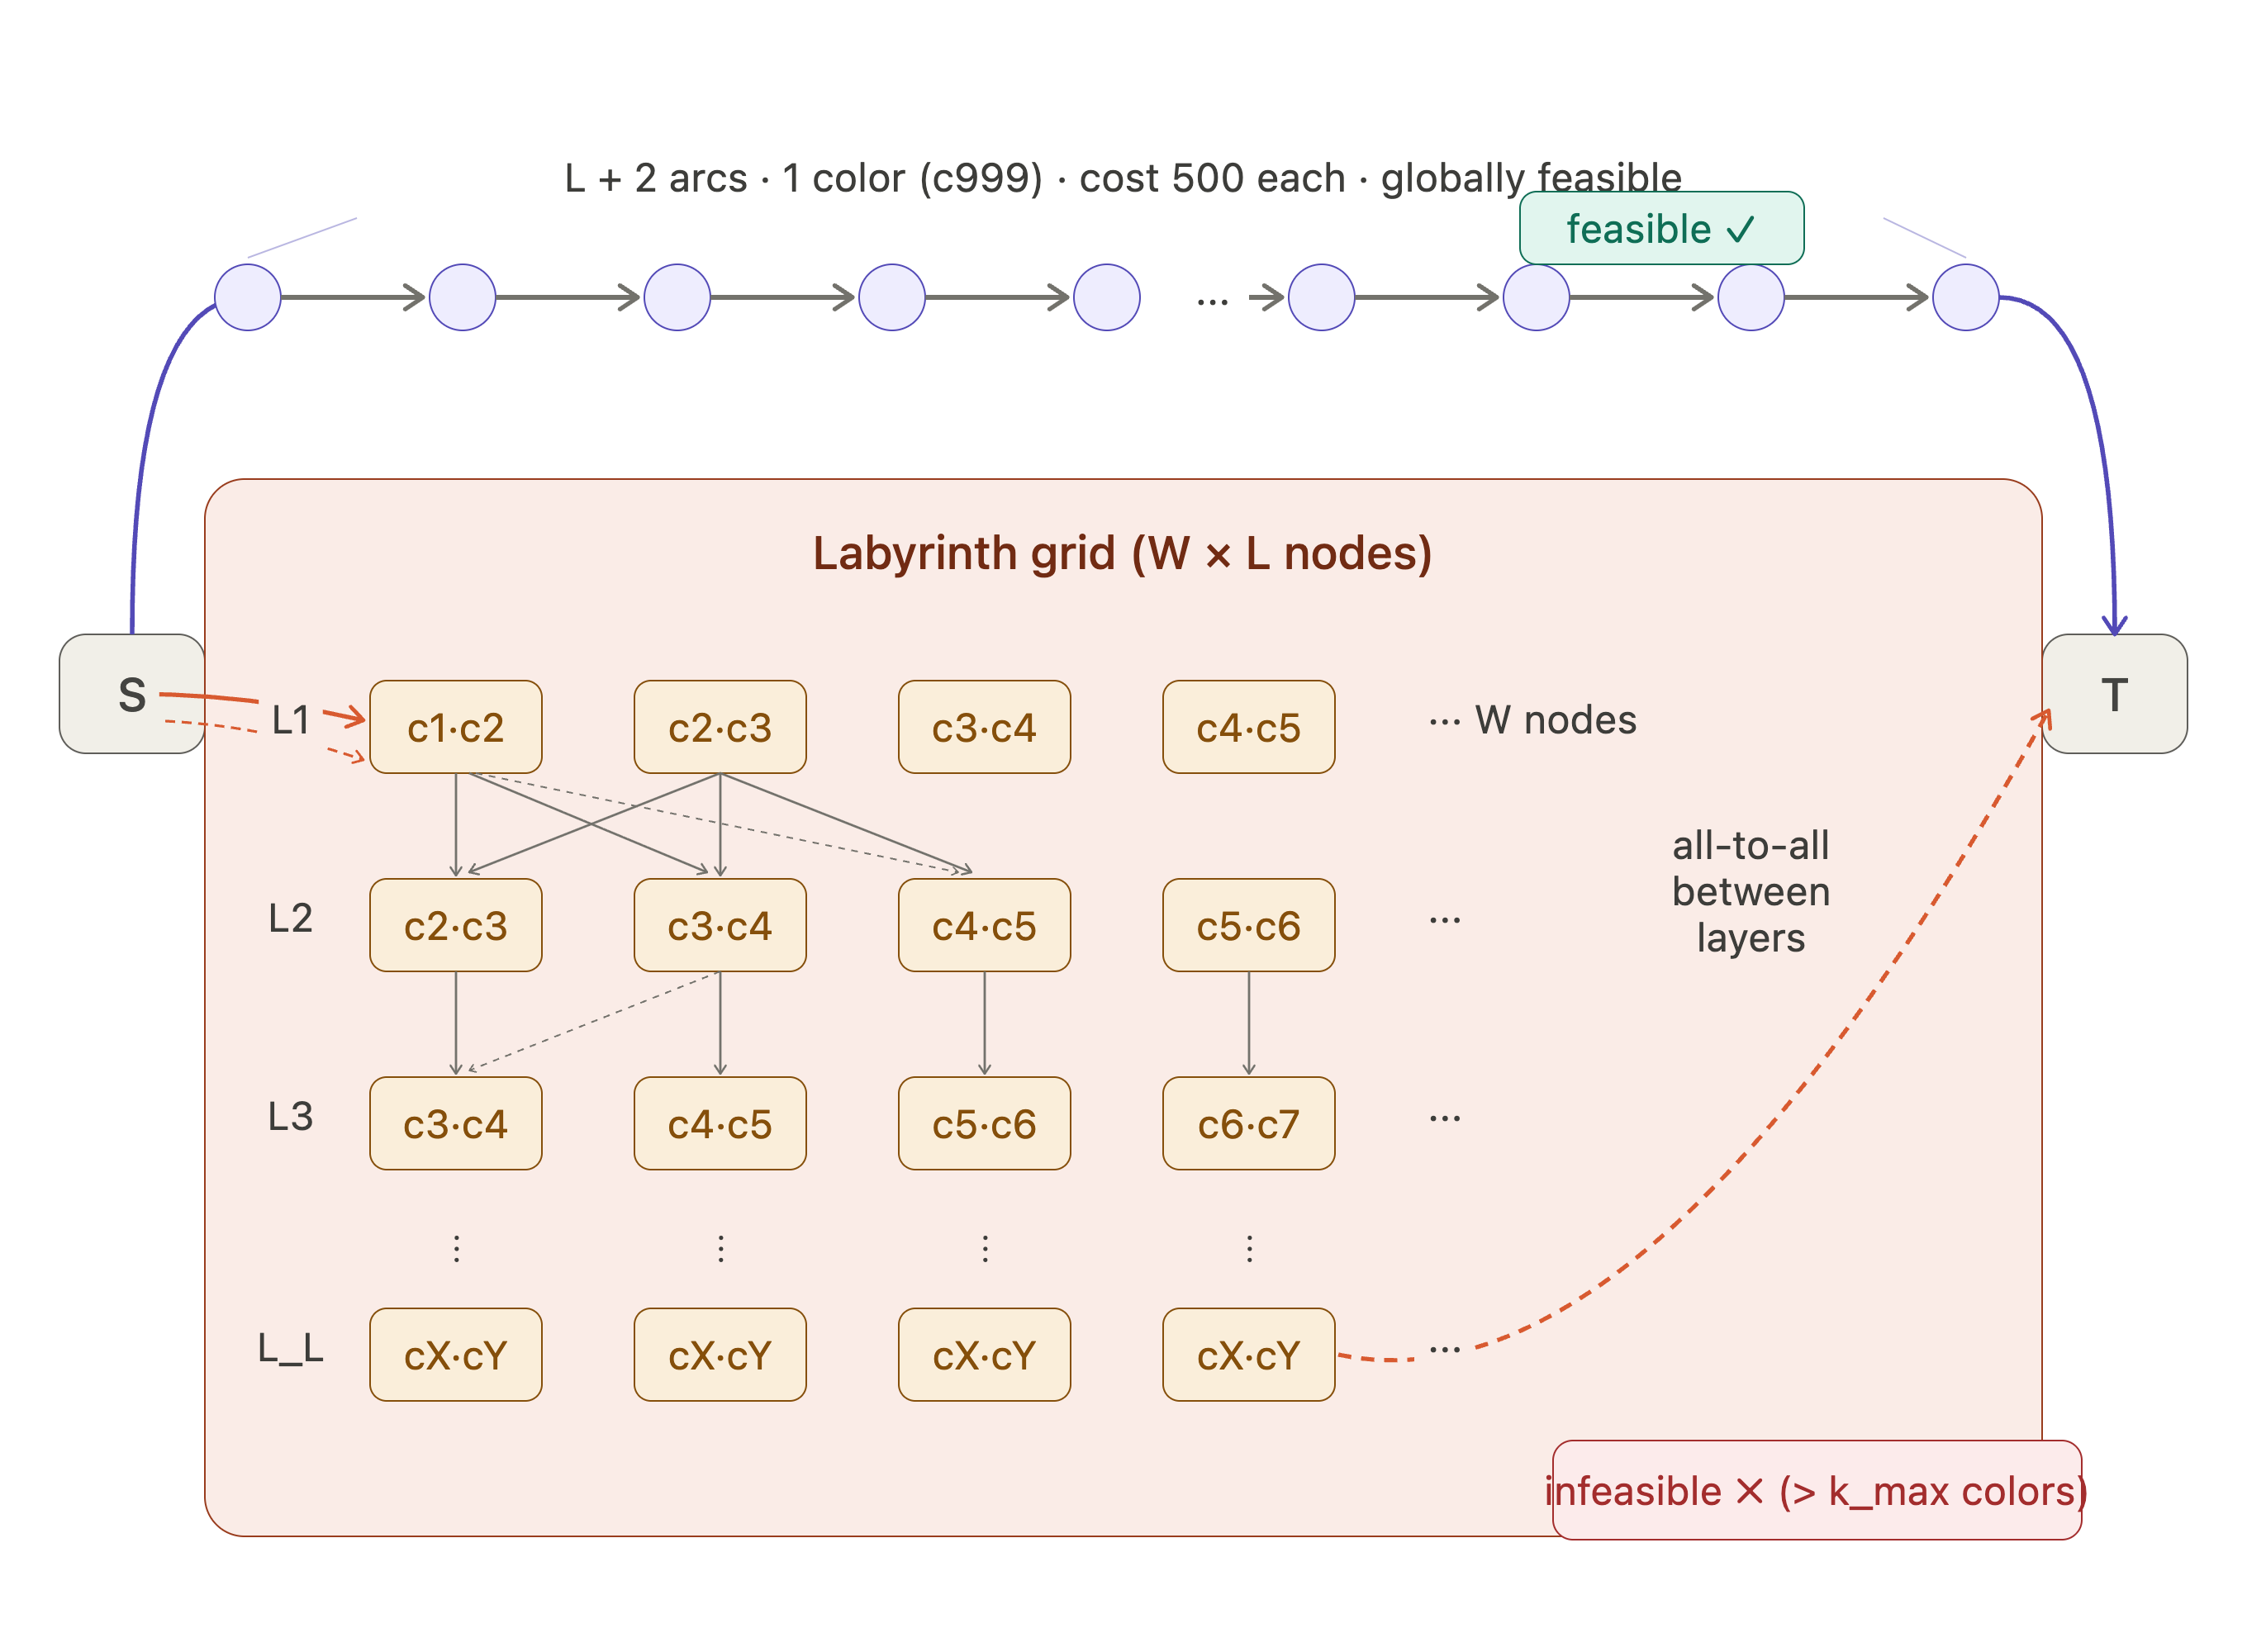
\includegraphics[width=0.9\textwidth]{charts/fractional_labyrinth_instance.png}
    \caption{Example of a labyrinth instance: two disjoint paths from $s$ to $t$, where the grid path introduces one new color per layer.}
     \label{fig:fractional_labyrinth_instance}
\end{figure}



\begin{table}[htbp]
\centering
\caption{Details about the benchmark instances for random and grid digraphs (Ferone et al., 2019).}
\label{tab:ferone-instances}
\begin{tabular}{lrrrrclrrrrr}
\toprule
\multicolumn{6}{c}{Random} & \multicolumn{6}{c}{Grid} \\
\cmidrule(r){1-6}\cmidrule(l){7-12}
\textit{inst} & $|V|$ & $|A|$ & $|R(A)|$ & $k$ & \textit{opt} &
\textit{inst} & $|V|$ & $|A|$ & $|R(A)|$ & $k$ & \textit{opt} \\
\midrule
% ---- Random R1 ----
R1-27190 & 75\,000 & 750\,000 & 16      & 8 & 242 &
   G1-27001 & 10\,000 & 39\,600 & 210    & 197 & 6\,233 \\
R1-27191 & 75\,000 & 750\,000 & 39      & 6 & 201 &
    G1-27003 & 10\,000 & 39\,600 & 444    & 196 & 6\,203 \\
R1-27195 & 75\,000 & 750\,000 & 13      & 6 & 152 &
  G1-27004 & 10\,000 & 39\,600 & 272    & 195 & 6\,375 \\
R1-27197 & 75\,000 & 750\,000 & 12      & 6 & 253 &
  G1-27007 & 10\,000 & 39\,600 & 223    & 198 & 6\,197 \\
R1-27199 & 75\,000 & 750\,000 & 48\,383 & 5 & 333 &
  G1-27008 & 10\,000 & 39\,600 & 215    & 191 & 6\,193 \\
R1-27200 & 75\,000 & 750\,000 & 143     & 6 & 236 &
  G1-27009 & 10\,000 & 39\,600 & 255    & 196 & 6\,183 \\
% ---- Random R3 ----

  
R3-27004 & 75\,000 & 750\,000 & 29      & 6 & 246 &
  G4-27000 & 62\,500 & 498\,500 & 859 & 767 & 23822 \\
R3-27005 & 75\,000 & 750\,000 & 25      & 6 & 198 &
  G4-27002 & 62\,500 & 498\,500 & 1209 & 770 & 23746 \\
R3-27007 & 75\,000 & 750\,000 & 38      & 6 & 231 &
  G4-27003 & 62\,500 & 498\,500 & 910 & 767 & 23610 \\
R3-27008 & 75\,000 & 750\,000 & 15      & 7 & 196 &
  G4-27004 & 62\,500 & 498\,500 & 1159 & 774 & 23904 \\
R3-27010 & 75\,000 & 750\,000 & 178     & 5 & 246 &
  G4-27005 & 62\,500 & 498\,500 & 883 & 773 & 23995 \\
R3-27012 & 75\,000 & 750\,000 & 28      & 7 & 245 &
  G4-27006 & 62\,500 & 498\,500 & 1519 & 762 & 23940 \\
\bottomrule
\end{tabular}
\end{table}

\begin{table}[htbp]
\caption{Details about the benchmark instances for layered-based digraphs (Castro et al., 2024) and the newly generated instances.}
\label{tab:unified-instances}
\small
\setlength{\tabcolsep}{6pt}
\begin{tabular}{lrrrrr@{\hspace{12pt}}lrrrrr}
\toprule
\multicolumn{6}{c}{Layered-based (Castro et al., 2024)} & \multicolumn{6}{c}{Newly generated instances} \\
\cmidrule(r){1-6}\cmidrule(l){7-12}
\textit{inst} & $|V|$ & $|A|$ & $|R(A)|$ & $k$ & \textit{opt} & 
\textit{inst} & $|V|$ & $|A|$ & $|R(A)|$ & $k$ & \textit{opt} \\
\midrule
GP1-3  & 152 & 1\,420 & 1\,420 & 7 & 5\,953 &  N-6 &   528 &   9\,667 &   9\,640 &  4 & 260.0 \\
GP1-4  & 152 & 1\,420 & 1\,420 & 7 & 5\,056 &  N-8 & 1\,088 &  30\,697 &  30\,660 & 20 & 360.0 \\
GP2-22 & 152 & 1\,447 & 1\,447 & 7 & 6\,211 &  N-9 & 1\,438 &  54\,517 &  54\,480 & 30 & 360.0 \\
GP2-23 & 152 & 1\,439 & 1\,430 & 7 & 5\,897 &  N-10 & 2\,298 & 110\,147 & 110\,100 & 40 & 460.0 \\
GP2-40 & 152 & 1\,440 & 1\,434 & 7 & 6\,845 & N-11 & 3\,358 & 194\,577 & 194\,520 & 50 & 560.0 \\
\bottomrule
\end{tabular}
\end{table}

\subsection{Results for DP, BDP, CPLEX, Valid Inequalities}

In Table \ref{tab:numerical_results_ferone}, we show the numerical results for the benchmark instance for random and grid digraph using the Dynamic Programming procedure with the $A^*$ extraction policy (Ferone et al. 2019 \cite{Ferone2021}), 
CPLEX solver with the CCDA \cite{CerroneRusso2023} heuristic solution
as a cutoff value, our implementation of the FFP model restricted to valid inequalities (17), (18), and (19) from (Castro et al. 2024\cite{Castro2024}) and finally our BDP solution.

The table also reports the CCDA upper bound (\textit{ub}) calculated for every \textit{instance}. The computational time (\textit{cpu}) is reported in seconds.
The (-) indicates the algorith reached the time limit or ran out of memory.
Each group (R1, R3, G1, G4) is separated by horizontal line, to calculate the statistics values Average, Median, Max and Min of every group.

The same legend has been used for layered-based digraph (Table \ref{tab:numerical_results_castro}) and the new-generated instances (Table \ref{tab:numerical_results_new}).

As already known from the literature \cite{Ferone2021} the DP algorithm performs well on average in the random/grid graph, there is some exception on some grid instance G1-27004 and G4-27000. 

The BDP approach achieves similar performance on the random digraph, showing a better median values for the grids groups (G1 and G4).
Regarding the layered-base digraphs (Table \ref{tab:numerical_results_castro})
both the DP and BDP algorithms suffer from combinatorial explosion due to the topology of this type of the graph and the $k$ which is set as the MCPP, this forces the process to explore all the
combination until the ends, pruning very few labels at each time.

With the newly generated (Table \ref{tab:numerical_results_new}) instances, because 
the labyrinth (Figure \ref{fig:fractional_labyrinth_instance}) introduces only 1 new color per layer, 
the DP must travel $k_{max} + 1$ layers deep into the grid before a path finally accumulates enough colors to trigger the cutoff.
BDP enters to the labyrinth from both sides simultaneously and only does half of the work on the optimal path.

The IBM CPLEX with the fixed $\textit{ub}$, turns out to be a bit slower than DP and BDP in the random graph on average, but 
has results in a fastest execution on grid digraph. Regarding the layered-base digraph were all solved to the optimality with an average time of 26.46 seconds.
The new instances have been resolved, but as the Graph grows in the depth, it starts to performs badly, because
there are exactly $k_{max}$ colors per layer, the fractional flow passing through any specific color $h$ is exactly $1/k_{max}$.
This forces the LP relaxation to split the unit flow of $1.0$ across the width of the grid.

Concerning the B\&C strategies with Valid Inequalities, as is known from the literature \cite{Castro2024} it performs well on average both random, grid digraph and layered digraph.
The strongest valid inequalities state that the sum of the flow on edges of color $h$ in a certain cut or non-reachable subset must be $\le y_h$ (the color activation variable). 
CPLEX perfectly satisfies all these complex cuts by setting the fractional variable $y_h = 1/k_{max}$.
Once CPLEX realizes the variables are fractional ($0.2$) and not binary ($0$ or $1$), it initiates the Branch-and-Bound phase. 
However, because the grid contains millions of perfectly symmetrical paths, there is no "best direction" to branch on. 
The solver gets lost exploring an exponentially large search tree of identical fractional values until the timeout.

\begin{table}[htbp]
\centering
\caption{Numerical results for DP, BDP, CPLEX, and Valid Inequalities for random and grid digraphs (Ferone et al., 2019)}
\label{tab:numerical_results_ferone}
\begin{tabular*}{\textwidth}{l@{\extracolsep{\fill}}rrrrr}
\toprule
\textit{Instance} & \multicolumn{1}{c}{CCDA} & \multicolumn{1}{c}{DP} & \multicolumn{1}{c}{BDP} & \multicolumn{1}{c}{CPLEX} & \multicolumn{1}{c}{Inequalities} \\
\cmidrule(lr){2-2} \cmidrule(lr){3-3} \cmidrule(lr){4-4} \cmidrule(lr){5-5} \cmidrule(lr){6-6}
 & \multicolumn{1}{c}{$ub$} & \multicolumn{1}{c}{$cpu$} & \multicolumn{1}{c}{$cpu$} & \multicolumn{1}{c}{$cpu$} & \multicolumn{1}{c}{$cpu$} \\
\midrule
R1--27190 & 242 & 0.0012 & 0.0125 & 0.5218 & 0.0196 \\
R1--27191 & 201 & 0.0011 & 0.0136 & 0.1089 & 0.0175 \\
R1--27195 & 152 & 0.0010 & 0.0057 & 0.1092 & 0.0161 \\
R1--27197 & 253 & 0.0011 & 0.0061 & 0.0952 & 0.0146 \\
R1--27199 & 333 & 0.1189 & 0.1373 & 2.4469 & 2.9082 \\
R1--27200 & 236 & 0.0014 & 0.0062 & 0.1265 & 0.0184 \\
\midrule
Average & 236.2 & \textbf{0.0208} & \textbf{0.0302} & 0.5681 & 0.4991 \\
Median & 239.0 & 0.0011 & 0.0094 & 0.1179 & 0.0180 \\
Max & 333.0 & 0.1189 & 0.1373 & 2.4469 & 2.9082 \\
Min & 152.0 & 0.0010 & 0.0057 & 0.0952 & 0.0146 \\
\midrule
R3--27004 & 246 & 0.0011 & 0.0060 & 0.1187 & 0.0173 \\
R3--27005 & 198 & 0.0011 & 0.0058 & 0.1169 & 0.0169 \\
R3--27007 & 231 & 0.0011 & 0.0057 & 0.1069 & 0.0175 \\
R3--27008 & 196 & 0.0013 & 0.0058 & 0.1366 & 0.0166 \\
R3--27010 & 246 & 0.0012 & 0.0061 & 0.1186 & 0.0180 \\
R3--27012 & 245 & 0.0011 & 0.0058 & 0.1226 & 0.0177 \\
\midrule
Average & 234.2 & \textbf{0.0021} & 0.0104 & 0.1229 & 0.0179 \\
Median & 238.0 & 0.0011 & 0.0060 & 0.1215 & 0.0177 \\
Max & 289.0 & 0.0098 & 0.0275 & 0.1417 & 0.0207 \\
Min & 196.0 & 0.0011 & 0.0057 & 0.1069 & 0.0166 \\
\midrule
G1--27001 & 6233 & 0.0002 & 0.0007 & 0.0073 & 0.0018 \\
G1--27003 & 6203 & 0.0026 & \textbf{0.0011} & 0.0135 & 0.0045 \\
G1--27004 & 6375 & 45.2761 & \textbf{0.0016} & 0.0082 & 0.0027 \\
G1--27007 & 6197 & 0.0007 & 0.0008 & 0.0072 & 0.0017 \\
G1--27008 & 6193 & 0.0003 & 0.0008 & 0.0074 & 0.0017 \\
G1--27009 & 6183 & 0.0006 & 0.0009 & 0.0080 & 0.0024 \\
\midrule
Average & 6205.8 & 7.0713 & 0.0331 & 0.0105 & 0.0038 \\
Median & 6195.0 & 0.0016 & \textbf{0.0014} & 0.0080 & 0.0024 \\
Max & 6375.0 & 45.2761 & 0.3080 & 0.0286 & 0.0154 \\
Min & 6079.0 & 0.0002 & 0.0007 & 0.0072 & 0.0017 \\
\midrule
G4--27000 & 23822 & 16.3234 & 0.0267 & 0.1595 & 0.0210 \\
G4--27004 & 23914 & 0.1367 & 127.8307 & 0.1238 & 0.0376 \\
G4--27005 & 23995 & 0.0273 & 0.0499 & 0.1397 & 0.0279 \\
G4--27006 & 23940 & - & 11.3697 & 0.1356 & 0.0326 \\
G4--27007 & 23953 & 0.0928 & 0.0180 & 0.1225 & 0.0215 \\
G4--27009 & 23798 & 0.3283 & 0.0162 & 0.1049 & 0.0185 \\
\midrule
Average & 23903.7 & 3.3817 & 23.2185 & 0.1310 & \textbf{0.0265} \\
Median & 23927.0 & 0.1367 & \textbf{0.0383} & 0.1297 & \textbf{0.0247} \\
Max & 23995.0 & 16.3234 & 127.8307 & 0.1595 & 0.0376 \\
Min & 23798.0 & 0.0273 & 0.0162 & 0.1049 & 0.0185 \\
\bottomrule
\end{tabular*}
\end{table}

\begin{table}[htbp]
\centering
\caption{Numerical results for DP, BDP, CPLEX, and Valid Inequalities for layered-based digraphs (Castro et al., 2024)}
\label{tab:numerical_results_castro}
\begin{tabular*}{\textwidth}{l@{\extracolsep{\fill}}rrrrr}
\toprule
\textit{Instance} & \multicolumn{1}{c}{CCDA} & \multicolumn{1}{c}{DP} & \multicolumn{1}{c}{BDP} & \multicolumn{1}{c}{CPLEX} & \multicolumn{1}{c}{Valid Inequalities} \\
\cmidrule(lr){2-2} \cmidrule(lr){3-3} \cmidrule(lr){4-4} \cmidrule(lr){5-5} \cmidrule(lr){6-6}
 & \multicolumn{1}{c}{$ub$} & \multicolumn{1}{c}{$cpu$} & \multicolumn{1}{c}{$cpu$} & \multicolumn{1}{c}{$cpu$} & \multicolumn{1}{c}{$cpu$} \\
\midrule
GP1-3 & - & - & - & 26.9545 & 2.3358 \\
GP1-4 & - & - & - & 2.9353 & 1.6920 \\
GP2-22 & 51145 & - & - & 23.8463 & 1.9515 \\
GP2-23 & 27388 & - & - & 19.4913 & 2.3121 \\
GP2-40 & 27264 & - & - & 59.0637 & 13.7712 \\
\midrule
Average & 35265.7 & - & - & 26.4582 & \textbf{4.4125} \\
Median & 27388.0 & - & - & 23.8463 & 2.3121 \\
Max & 51145.0 & - & - & 59.0637 & 13.7712 \\
Min & 27264.0 & - & - & 2.9353 & 1.6920 \\
\bottomrule
\end{tabular*}
\end{table}

\begin{table}[htbp]
\centering
\caption{Numerical results for DP, BDP, CPLEX, and Valid Inequalities (New Instances)}
\label{tab:numerical_results_new}
\begin{tabular*}{\textwidth}{l@{\extracolsep{\fill}}rrrrr}
\toprule
\textit{Instance} & \multicolumn{1}{c}{CCDA} & \multicolumn{1}{c}{DP} & \multicolumn{1}{c}{BDP} & \multicolumn{1}{c}{CPLEX} & \multicolumn{1}{c}{Valid Inequalities} \\
\cmidrule(lr){2-2} \cmidrule(lr){3-3} \cmidrule(lr){4-4} \cmidrule(lr){5-5} \cmidrule(lr){6-6}
 & \multicolumn{1}{c}{$ub$} & \multicolumn{1}{c}{$cpu$} & \multicolumn{1}{c}{$cpu$} & \multicolumn{1}{c}{$cpu$} & \multicolumn{1}{c}{$cpu$} \\
\midrule
N-6  & 260 & 0.0261 & 0.0001 & 0.9947 & 1.6116 \\
N-8  & 360 & - & 0.0001 & 6.1689 & 1.9709 \\
N-9  & 360 & - & 0.0001 & 5.5231 & 5.6575 \\
N-10 & 460 & - & 0.0002 & 40.1596 & 16.6383 \\
N-11 & 560 & - & 0.0003 & 377.3205 & 42.2813 \\
\midrule
Average & 400.0 & 0.0261 & \textbf{0.0002} & 86.0334 & 13.6319 \\
Median  & 360.0 & 0.0261 & 0.0001 & 6.1689 & 5.6575 \\
Max     & 560.0 & 0.0261 & 0.0003 & 377.3205 & 42.2813 \\
Min     & 260.0 & 0.0261 & 0.0001 & 0.9947 & 1.6116 \\
\bottomrule
\end{tabular*}
\end{table}

\section{Conclusions and future works}
This project proposed and evaluated a bounded bi-directional dynamic programming (BDP) approach to solve the NP-hard $k$-color Shortest Path Problem ($k$-CSPP). 
By extending labels simultaneously from the source and destination nodes and utilizing a half-way stopping criterion based on an upper bound heuristic, the BDP algorithm effectively limits redundant label generation. 

Computational experiments demonstrate that BDP maintains competitive execution times on standard random and grid graphs, often achieving better median performance than standard dynamic programming. 
Furthermore, on newly generated labyrinth instances BDP significantly outperformed both mono-DP and Valid Inequalities by halving 
the required search space and quickly identifying path infeasibilities.  
Despite these improvements, layered-based digraphs remain exceptionally challenging for dynamic programming techniques due to severe combinatorial explosion. 

Future improvements could include integrating other bounding techniques like State Space Relaxation, Decremental State Space Relaxation or NG-routes relaxation that could reduce the exploration,
even though the non-additive property of the colors is important limit to take into account. 
\bibliography{references}

\end{document}